\documentclass[11pt,a4paper]{report} 

% Für doppelseitigen Ausdruck (nur bei > 60 Seiten sinnvoll)
% \usepackage{ifthen}
% \setboolean{@twoside}{true}
% \setboolean{@openright}{true} 

\include{preamble} % alle Pakete und Einstellungen

% Hier anpassen 
%\newcommand{\welchethesis}{Bachelor}
\newcommand{\welchethesis}{Master}
\newcommand{\thesisofwas}{of Science}
%\newcommand{\studiengang}{Technische Informatik}
% \newcommand{\studiengang}{Medizintechnik}
\newcommand{\studiengang}{Informationstechnik}
\newcommand{\titel}{Compositional Gaussian Splatting for Multi-Object and Dynamic Scene
Synthesis}
\newcommand{\kurztitel}{Compositional Gaussian Splatting}
\newcommand{\autor}{Luca Hebeda}
\newcommand{\datum}{31. Oktober 2025} % Abgabedatum
\newcommand{\ort}{Mannheim}
\newcommand{\hochschullehrer}{Prof.\ Dr.\ Marcus Vetter}
\newcommand{\zweikorrektor}{M. Sc. Yannick Bukschat}

\begin{document}
\begin{titlepage}
  % Kopf der Seite
  \parbox[b]{80mm}{
    % \textsf würde das Aussehen der ersten Seite ruinieren, 
    % wer will, soll das selbst außen rum machen...
    Department of Information Technology\\
    Course of Studies: \studiengang}
  \hfill
  \parbox[b]{42mm}{\includegraphics[width=42mm,valign=c,raise=3mm]{images/thmannheimlogo_grey.pdf}}
  \begin{center}
    % rumfiddeln, damit es für 4 Zeilen gerade noch so geht...
    \rule{1\textwidth}{1pt}\\[-3mm]
    \parbox[t][64mm]{110mm}{% 11 cm für Breite 13, ca. 7 für Höhe 6
      \begin{center}
        \vspace{6mm}
        %\Large{Master Thesis}\\[2mm]
        {\begin{spacing}{1.13} \huge \bfseries \titel \end{spacing}}
        \vfill
        \Large{\autor} \\[1mm] % keep space to window
        \ 
      \end{center}
    }
    \rule{\textwidth}{1pt}    
    \vfill    
    {\Large Master Thesis} \\[5mm]
    {\large for the acquisition of the academic degree} \\[5mm]
    {\large \welchethesis\ \thesisofwas} \\[5mm]
    \vfill    
    % \begin{tabular}{ll} % Mitte der Seite
    %   Vorgelegt von & \autor \\
    %   am & \datum \\
    %   Hochschullehrer/in & \hochschullehrer \\
    %   Zweikorrektor/in & \zweikorrektor
    % \end{tabular}    
    \begin{tabular}{ll}
    Submitted by & \autor \\
    on & \datum \\
    Supervisor & \hochschullehrer \\
    Second examiner & \zweikorrektor
    \end{tabular}   
    \vfill
  \end{center}
\end{titlepage}
\cleardoublepage


% Erklärung gemäß der Prüfungsordnung
\thispagestyle{empty}

\subsection*{Written Declaration in Accordance with the Study and Examination Regulations}

  I hereby declare that I have written this thesis independently and have not used any sources or aids other than those indicated.  
  All passages that are taken literally or in substance from other works are identified as such.  

% \subsection*{Schriftliche Versicherung laut Studien- und Prüfungsordnung}

% Hiermit erkläre ich, dass ich die vorliegende Arbeit selbstständig verfasst
% und keine anderen als die angegebenen Quellen und Hilfsmittel benutzt habe.

\vspace{6em}
\noindent\begin{tabular}{p{0.37\textwidth}p{0.56\textwidth}}
\ort, \datum  & \rule{0.56\textwidth}{0.5pt}\\
              & \makebox[1cm]{\ } \autor
\end{tabular}

\vfill

\cleardoublepage
 % Titelseite, Erklärungen, etc.

\begin{abstract}
We present a modular and methodologically transparent pipeline for multi-view and temporally consistent synthetic dataset generation based on Gaussian Splatting. 
The framework integrates static 3D Gaussian Splatting (3DGS) and persistent Dynamic 3D Gaussian Splatting (D3DGS) into a unified system that enables reconstruction, export, and recomposition of dynamic multi-object scenes. 
Using a hardware-synchronized 56-camera rig, we capture spatially dense and temporally aligned sequences that serve as the basis for static background reconstruction and dynamic object modeling. 
A dedicated compositing stage allows the exported Gaussian models to be reinserted, duplicated, or combined into novel virtual environments, producing multi-view renderings with synchronized RGB, depth, segmentation, and occlusion annotations. 
Additional modules provide pose estimation, keypoint propagation, and temporal supersampling for motion-consistent supervision signals. 
Qualitative evaluations demonstrate that the pipeline maintains spatial coherence, robust occlusion reasoning, and temporal stability across views and environments. 
The system establishes a practical foundation for controllable 4D dataset generation and for benchmarking methods in dynamic scene understanding.
\end{abstract}


\tableofcontents

\onehalfspacing

% \linenumbers
\section{Introduction}

\subsection{Motivation}
Artificial intelligence has made remarkable progress in understanding and generating visual content \cite{lecun2015deep, krizhevsky2012imagenet}. Modern computer vision systems can recognize objects, estimate depth, and reconstruct three-dimensional scenes from ordinary images \cite{he2017mask, zollhoefer2018state}. At the core of these capabilities lies the data used to train and evaluate such models \cite{sun2017revisiting}. Most deep learning approaches rely on large collections of labeled data, yet creating high-quality datasets with accurate geometry and temporal consistency remains one of the most expensive and time-consuming aspects of research and development \cite{everingham2010pascal, lin2014microsoft}.

In recent years, visual scene representation has shifted from traditional image-based techniques toward neural and hybrid three-dimensional representations. Neural scene representation aims to describe a scene not as a set of disconnected pixels but as a continuous spatial structure that can be observed from any viewpoint \cite{mildenhall2021nerf}. Methods such as Neural Radiance Fields (NeRFs) have shown that continuous three-dimensional models can be reconstructed from ordinary photographs, although these methods often involve long optimization times and complex rendering processes \cite{barron2021mip}.

Gaussian Splatting has recently emerged as a faster and more transparent alternative \cite{kerbl3Dgaussians}. Instead of relying on deep implicit functions, it models a scene as a collection of Gaussian primitives representing color, position, and opacity in space. This approach allows real-time rendering while maintaining a high level of detail and realism \cite{fridovich2023k}. Because Gaussian primitives can be easily manipulated and recombined, they offer new possibilities for modular scene generation and synthetic data creation \cite{CutAndSplat2024}.

The generation of synthetic data is increasingly important for artificial intelligence \cite{tobin2017domain, denninger2019blenderproc}. Real-world datasets are often limited by annotation errors, missing labels, and insufficient diversity \cite{dwibedi2017cutpaste}. Synthetic datasets can overcome these limitations by providing unlimited, precisely labeled, and perfectly synchronized examples \cite{zanjani2025gaussian}. They are particularly valuable in scenarios where ground-truth information such as depth, motion, or segmentation is difficult to obtain manually \cite{godard2017unsupervised, bertasius2019maskprop}.

For training robust AI models, both the quality and diversity of data are critical. A system that can automatically generate realistic, correctly annotated images from structured three-dimensional representations thus offers significant advantages for both academic research and industrial applications.

Despite this potential, most existing methods focus on reconstructing individual static or dynamic scenes \cite{luiten2024dynamic,yang2024deformable}, without providing tools for composing multiple objects or actors into coherent multi-view environments with synchronized annotations. Many practical applications—such as robotics, autonomous systems, and simulation—require dynamic scenes that include interacting elements while maintaining accurate geometry and temporal alignment \cite{CutAndSplat2024}.

\subsection{Structure of the Work}
This thesis addresses the aforementioned challenges by developing a modular pipeline based on static and dynamic Gaussian Splatting. The proposed system enables the reconstruction, composition, and rendering of complex multi-object scenes in calibrated camera setups. It produces synchronized outputs including color images, depth maps, and instance-level segmentation. Additionally, the framework supports annotations such as keypoints, occlusion scores, and estimated poses, providing a comprehensive solution for generating structured and reproducible synthetic datasets.

The approach emphasizes compositional reliability rather than algorithmic novelty. By integrating existing Gaussian Splatting methods into a unified workflow, it demonstrates how realistic and temporally consistent synthetic data can be generated with minimal manual effort. In this way, the system bridges the gap between recent advances in neural scene representation and the practical need for scalable dataset generation.

The remainder of this thesis is organized as follows. Chapter~\ref{chap:Fundamentals} introduces the theoretical foundations of Gaussian Splatting. Chapter~\ref{chap:State_of_the_Art} reviews existing methods and positions the proposed system within the broader landscape of Gaussian-based representations and related work in dynamic scene modeling, including a detailed discussion of the two most prominent approaches. Chapter~\ref{chap:Methodology} describes the modifications and training improvements applied, followed by a step-by-step presentation of the completed pipeline. Chapter~\ref{chap:Results} presents reconstruction results for both static and dynamic Gaussian Splatting and provides a qualitative evaluation of the newly constructed pipeline. Finally, Chapter~\ref{chap:Conclusion} summarizes the key findings, discusses limitations, and outlines potential directions for future research.
 % Externe Datei einbinden
\chapter{Fundamentals}
\label{chap:Fundamentals}

The following chapter explains the fundamental theoretical concepts required to understand this thesis.


\section{Neural Radiance Fields}
\label{sec:Fundamentals_NeRF}

Neural Radiance Fields (NeRF), introduced by Mildenhall et al. \cite{mildenhall2021nerf}, represent a decisive step in the development of novel 3D scene representations.
The approach models a scene implicitly through a neural network that predicts volumetric density and color for a given position and viewing direction.
By employing differentiable rendering techniques and optimizing on multi-view image data, it becomes possible to reconstruct novel viewpoints with high quality.
The underlying idea is illustrated in Figure \ref{fig:nerf_teaser}.

\begin{figure}[h]
    \centering
    \includegraphics[width=1\linewidth]{Grafiken/Fundamentals/teaser_small.pdf}
    \caption{Core principle of NeRF: A model is optimized from input images and can subsequently generate novel views of the scene (after \cite{mildenhall2021nerf}).}
    \label{fig:nerf_teaser}
\end{figure}

The model receives a 5D vector \((x, y, z, \theta, \phi)\) as input, consisting of the 3D position and the ray direction. 
For each combination of position and direction, the MLP outputs a value for density \(\sigma\) and the associated color \((r, g, b)\).
Rendering is performed by integrating the color and density values estimated by NeRF along the rays projected from the camera into the scene.
The scene representation is optimized by minimizing the photometric error between the rendered and the actual image.
The pipeline is illustrated in Figure \ref{fig:nerf_pipeline}.

\begin{figure}[h]
    \centering
    \includegraphics[width=1\linewidth]{Grafiken/Fundamentals/pipeline.pdf}
    \caption{NeRF pipeline: The MLP maps 5D inputs to color and density, which are composed into an image via volumetric rendering (after \cite{mildenhall2021nerf}).}
    \label{fig:nerf_pipeline}
\end{figure}

NeRF enables detailed reconstruction and accurate depiction of complex lighting effects such as reflections and transparencies, making it particularly suitable for photorealistic applications.
Furthermore, the implicit representation ensures consistent multi-view renderings that allow robust synthesis of novel perspectives.


\section{Gaussian Splatting}

While NeRF enables high rendering quality, it suffers from long training times and slow rendering, which is particularly problematic for dynamic scenes and interactive applications.
This motivated the development of alternative representations that are more explicit and efficient.
One of the most significant works in this area is 3D Gaussian Splatting (3DGS) by Kerbl et al. \cite{kerbl3Dgaussians}.
The approach replaces NeRF’s implicit network representation with a set of explicit 3D Gaussians that can be rendered in real time while maintaining high image quality.
An overview of this approach is shown in Figure \ref{fig:overview}, which illustrates the optimization and rendering pipeline of Gaussian Splatting.
The following sections discuss the detailed components of this model to provide a comprehensive understanding of its operation.

\begin{figure*}
\centering
\includegraphics[width=\linewidth]{Grafiken/Fundamentals/overview_01.pdf}
\caption{Optimization and rendering pipeline of Gaussian Splatting: The process begins with a sparse structure-from-motion (SfM) point cloud, which serves as the basis for creating an initial set of 3D Gaussian functions. These Gaussians are refined through iterative optimization, with their density adaptively controlled to ensure accurate scene representation. A fast tile-based rasterizer enables competitive rendering times compared to modern radiance field methods (figure from \cite{kerbl3Dgaussians}).}
\label{fig:overview}
\end{figure*}


\subsection{Scene Representation with 3D Gaussians}

In contrast to NeRF, which requires images from multiple viewpoints as well as camera poses from multi-view stereo (MVS) \cite{schoenberger2016mvs}, Gaussian Splatting is based on a sparse point cloud and camera poses obtained via structure-from-motion (SfM) techniques such as COLMAP \cite{schoenberger2016sfm}.
These points form the basis for creating a set of 3D Gaussian functions, each defined by its position (\(\mu\)), an anisotropic covariance matrix (\(\Sigma\)), an opacity (\(\alpha\)), and spherical harmonic coefficients for color representation.
The 3D Gaussian functions, referred to as \textit{3D Gaussians} throughout this work, are differentiable and can be efficiently projected into 2D splats, allowing fast \(\alpha\)-blending for rendering.
The 3D Gaussians are described by a covariance matrix \(\Sigma\) in world coordinates \cite{kerbl3Dgaussians}, which defines their shape and orientation in 3D space:

\begin{align}
G(x) = e^{-\frac{1}{2} x^T \Sigma^{-1} x}
\end{align}

The matrix \(\Sigma\) describes the extent and correlation of the Gaussian along different axes, providing a compact and flexible representation of the scene.
During rendering, each Gaussian is weighted by its opacity \(\alpha\) to contribute to the final image.


\subsection{Rendering with 3D Gaussian Splatting}

Rendering 3D Gaussians onto the 2D image plane requires several transformations and optimizations to ensure both accuracy and efficiency.
The approach proposed by Zwicker et al. \cite{zwicker2001ewa} provides a robust framework that is central to the 3D Gaussian Splatting technique.

\subsubsection{Projection of 3D Gaussians}

The projection of 3D Gaussians onto the 2D image plane is based on affine transformations and the computation of the covariance matrix in camera coordinates.
The original covariance matrix \(\Sigma\) describes the spatial distribution of the Gaussians in 3D space.
To project it onto the image plane, a view transformation \(W\) is applied, converting the covariance matrix into camera coordinates. The resulting transformed covariance matrix \(\Sigma'\) is computed as follows:

\begin{align}
\Sigma' = J W \Sigma W^T J^T
\end{align}

Where:
\begin{itemize}
    \item \(\Sigma'\): transformed covariance matrix in camera coordinates,
    \item \(W\): view transformation from world to camera coordinates,
    \item \(\Sigma\): original covariance matrix of the 3D Gaussian functions,
    \item \(J\): Jacobian matrix of the affine projection.
\end{itemize}

The Jacobian \(J\) describes the effect of the affine projection on small variations in 3D coordinates.
This transformation maps the spatial distribution of the Gaussians onto the 2D image plane, accounting for the uncertainty of the data points during rendering.

\subsubsection{Simplified Covariance Computation}

Since the transformation described above can be computationally expensive, a simplified approach is often used, based on scaling and rotation matrices.
The covariance matrix \(\Sigma\) can be expressed using a scaling matrix \(S\) and a rotation matrix \(R\):

\begin{align}
\Sigma = R S S^T R^T
\label{eq:calc_sigma}
\end{align}

For optimization, scaling and rotation are stored separately: a 3D vector \(s\) for scaling and a quaternion \(q\) for rotation.
These can easily be converted into matrices and combined, with the quaternion \(q\) being normalized to ensure a valid unit rotation.
This approach allows efficient computation and optimization of the 3D Gaussian Splatting parameters.


\subsection{Optimization}

Optimization in 3D Gaussian Splatting is based on iteratively rendering the scene and comparing it with training images to minimize projection errors of 3D structures on the 2D image plane.
The parameters of the 3D Gaussians, position ($\mu$), covariance matrix ($\Sigma$), opacity ($\alpha$), and color coefficients, are adjusted using stochastic gradient descent.
Opacity \(\alpha\) is constrained to the range [0, 1] using a sigmoid function, while covariance scaling is controlled with an exponential activation function.
The covariance matrix is initially estimated as an isotropic Gaussian model based on the distances to the three nearest points.

The optimization employs a combined loss function:

\begin{align}
\mathcal{L} = (1 - \lambda) \mathcal{L}_1 + \lambda \mathcal{L}_{\text{D-SSIM}}
\label{eq:loss_GS}
\end{align}

Here, \(\mathcal{L}_1\) measures absolute pixel differences between rendered and training images, while \(\mathcal{L}_{\text{D-SSIM}}\) evaluates structural similarity to preserve fine details.
The weighting factor \(\lambda\) balances these two components.

\subsubsection{Adaptive Control of 3D Gaussians}

Adaptive density control, illustrated in Figure \ref{fig:adaptivecontrol}, optimizes the number and distribution of 3D Gaussians.
Every 100 iterations, transparent Gaussians with \(\alpha < \epsilon_\alpha\) are removed, and in regions with large position-dependent gradients, small Gaussians are cloned or large ones are split into smaller ones to accurately represent geometry.
Every 3000 iterations, density is regularized by resetting \(\alpha\) values.
Large Gaussians with excessive influence are removed to maintain efficiency.
This approach allows for a compact and precise scene representation without additional spatial compression.

\begin{figure}[h]
\centering
\includegraphics[width=0.5\textwidth]{Grafiken/Fundamentals/density_control_01.pdf}
\caption{Adaptive density control: The top row shows under-reconstruction, where small geometries (black outlines) are supplemented by cloning a Gaussian. The bottom row shows over-reconstruction, where a large Gaussian is split into two smaller ones (after \cite{kerbl3Dgaussians}).}
\label{fig:adaptivecontrol}
\end{figure}


\subsection{Differentiable Rasterizer}

The differentiable rasterizer is central to efficient rendering and optimization of scenes in 3D Gaussian Splatting, as it enables real-time performance and high-quality image synthesis \cite{kerbl3Dgaussians}.

\subsubsection{Tile-based Rasterization Process}

The rasterization projects 3D Gaussians onto the 2D image plane using a view transformation.
The influence of each Gaussian on the pixel grid is computed based on its position (\(\mu\)), covariance (\(\Sigma\)), and opacity (\(\alpha\)).
A tile-based approach divides the image plane into small tiles processed in parallel on the GPU.
The Gaussians are sorted by depth, and their IDs are stored in a list.
Sorting ensures correct color and transparency values during the blending process.

\subsubsection{Rendering and Blending}

During the rendering stage, the individual contributions of all projected Gaussians are accumulated to synthesize the final image. 
Each Gaussian acts as a semi-transparent, view-dependent surface element whose influence on the pixel color is weighted by its opacity and spatial extent in image space. 
This process is realized through \(\alpha\)-blending, a differentiable compositing operation that models light accumulation along the viewing ray.

Formally, the color of a pixel is obtained by sequentially blending all \(N\) Gaussians along the ray in depth order:
\begin{align}
C = \sum_{i=1}^N T_i \alpha_i c_i, \quad \text{with} \quad T_i = \prod_{j=1}^{i-1} (1-\alpha_j)
\end{align}

Here, each term in the summation corresponds to a single Gaussian contribution:
\begin{itemize}
    \item \(C\): final accumulated pixel color,
    \item \(T_i\): transmittance describing how much light passes through all previous Gaussians,
    \item \(\alpha_i\): opacity of the \(i\)-th Gaussian, determining its visibility,
    \item \(c_i\): emitted color of the \(i\)-th Gaussian.
\end{itemize}

The transmittance term \(T_i\) ensures physically correct ordering along the ray, such that closer Gaussians partially occlude those behind them. 
This yields a continuous and differentiable approximation of volumetric compositing, analogous to classical volume rendering but without explicit ray integration.

For each pixel \((u, v)\), the color can be expressed more precisely as:
\begin{align}
I(u, v) = \sum_{i=1}^{N} p_i(u, v; \mu_i^{2d}, \Sigma_i^{2d}) \, \alpha_i \, c_i(d_i) \,
\prod_{j=1}^{i-1} \big(1 - p_j(u, v; \mu_j^{2d}, \Sigma_j^{2d}) \, \alpha_j \big)
\label{eq:projection_3D_gaussians} 
\end{align}

Here, \(p_i(u, v; \mu_i^{2d}, \Sigma_i^{2d})\) denotes the projected 2D Gaussian footprint on the image plane, which determines how strongly each Gaussian contributes to a given pixel.
The term \(c_i(d_i)\) models view-dependent color variations based on the viewing direction \(d_i\), typically parameterized through spherical harmonics. 
Finally, the product term \(\prod_{j=1}^{i-1} (1 - p_j \alpha_j)\) ensures correct visibility by progressively attenuating the contributions of Gaussians located behind others along the ray.


\subsubsection{Backward Pass and Gradient Computation}

Since the entire rendering pipeline is differentiable, gradients of the image reconstruction loss can be propagated back through the rasterization process. 
During the forward pass, the rasterizer stores intermediate quantities such as accumulated transmittance and per-pixel \(\alpha\)-values, which are reused in the backward pass to efficiently compute derivatives. 
This allows for the calculation of gradients with respect to Gaussian parameters including position \(\mu\), covariance \(\Sigma\), opacity \(\alpha\), and color coefficients.

By leveraging these stored buffers, the system avoids redundant recomputation of visibility and blending terms, substantially accelerating optimization. 
This differentiable rasterization design enables end-to-end training through standard gradient descent, directly optimizing the spatial distribution and appearance of Gaussians based on image-space supervision.

\chapter{State of the Art}

\section{Gaussian Splatting for Scene Representation}

Gaussian Splatting has recently emerged as a compact and efficient method for high-quality novel-view synthesis. It provides a practical alternative to volumetric or implicit representations such as Neural Radiance Fields.~\cite{mildenhall2021nerf,barron2021mip,barron2023zipnerf}. 
In GS, a scene is modeled as a set of anisotropic 3D Gaussian primitives, each parameterized by position, covariance, color, and opacity, which are projected and rasterized into image space. 

This representation provides both high rendering fidelity and real-time performance while avoiding the computationally expensive optimization and ray marching inherent to NeRF-based methods~\cite{kerbl3Dgaussians}. 
Because Gaussian primitives can be directly exported, edited, and recombined, 3DGS serves as a convenient intermediate representation for object-level modeling and downstream applications.
Recent studies have extended the approach with semantic and structural grouping of Gaussian primitives.
For instance, Gaussian Grouping~\cite{gaussian_grouping} demonstrated that semantically coherent clusters of Gaussians can be learned jointly with scene geometry, enabling object-level reasoning and segmentation directly in Gaussian space.
Such methods illustrate that Gaussian-based representations can serve as a unified bridge between geometric reconstruction and semantic scene understanding.

\section{Dynamic Extensions of Gaussian Splatting}

Following the success of static 3D Gaussian Splatting (3DGS), a substantial body of work has extended the approach to dynamic scenes. 
Two main paradigms have emerged.

The first models temporal evolution explicitly by tracking Gaussian primitives over time. 
Each Gaussian is associated with a trajectory describing its spatial and appearance changes, enabling temporal coherence without retraining. 
Early works such as \textit{Dynamic 3D Gaussians}~\cite{luiten2024dynamic} and \textit{Dynamic Gaussian Marbles}~\cite{stearnsmarbels} follow this paradigm, deriving dense motion fields from the per-Gaussian trajectories. 
More recent variants such as \textit{Deformable 3DGS}~\cite{yang2024deformable} incorporate deformation fields inspired by D-NeRF~\cite{pumarola2021d}, improving temporal smoothness and geometric consistency through explicit regularization. 
These methods preserve modularity and interpretability, allowing reconstructed objects to be reused and exported, but they require careful trajectory regularization to avoid drift.

The second paradigm embeds time directly into the Gaussian representation, treating the primitives as 4D entities with a temporal axis. 
Representative approaches include \textit{4DGS}~\cite{yang2023gs4d}, \textit{SpaceTime Gaussians}~\cite{lispacetimegaussianfeaturesplattingrealtime2024}, and \textit{4D Gaussian Splatting}~\cite{wu20244d}, which employ high-dimensional parameterizations or low-rank factorizations (e.g., K-Planes \cite{fridovich2023k}) to model spatio-temporal changes in position, scale, and orientation. 
These methods achieve globally consistent reconstructions across time but at the cost of increased computational demand and reduced flexibility. 
Once trained, 4DGS models are monolithic and difficult to segment, edit, or recombine, making them less suited for object-centric workflows or dataset generation.

From the perspective of dataset generation, the trajectory-based approach offers better modularity and reusability. It allows reconstructed objects to be relocated, duplicated, or combined across scenes, which is essential for large-scale synthetic data pipelines. Although four-dimensional representations achieve elegant temporal consistency, their high computational cost and limited flexibility make them less practical for compositional workflows. For this reason, the pipeline developed in this work adopts a trajectory-based dynamic formulation that balances temporal coherence with scalability and per-object control.

\section{Synthetic Compositing and Dataset Pipelines}

Parallel to developments in neural scene representations, a growing body of work addresses synthetic data generation for computer vision. 
Approaches vary from simple image-level composition to physically grounded 3D rendering pipelines. 
Some works create datasets by cutting out segmented objects and pasting them into real backgrounds, optionally guided by depth or matting networks~\cite{Dwibedi2017,Tobin2017,Liu2018,Li2023MattingSurvey}. 
Others synthesize entire virtual scenes using graphics engines such as BlenderProc or Unreal Engine, enabling precise control over scene layout, lighting, and annotations~\cite{Denninger2019,Lee2018}. 
More recent efforts combine learned 3D object models with image-based rendering to generate annotated imagery (RGB, depth, segmentation) for downstream tasks~\cite{Kirillov2023,Bertasius2020,Godard2019,Niu2021}.

However, many compositing pipelines still rely on 2D-level heuristics such as monocular depth estimation or per-frame segmentation, which introduce inconsistencies across viewpoints and over time~\cite{InpaintingLimitations2019,MonoDepthLimitations2018}. 
Promptable segmentation frameworks like SAM~\cite{Kirillov2023} have improved mask quality, but their integration into geometry-aware, multi-view pipelines remains limited~\cite{MaskPropagation2019}. 
Using explicit 3D representations—such as object-level Gaussian models—can mitigate these issues by preserving intrinsic spatial consistency and enabling deterministic occlusion reasoning across views.

Beyond masks and depth, many dataset pipelines incorporate mid-level cues such as 2D keypoints to provide additional semantic structure. 
Modern detectors based on Mask R-CNN and Detectron2 architectures~\cite{He2017MaskRCNN,Detectron22020} produce accurate joint locations but remain frame-dependent, often suffering from temporal jitter or occlusion failures. 
To improve stability, lightweight propagation and filtering techniques are applied to transfer reliable detections across time~\cite{MaskPropagation2019}. 

\section{Gaussian Splatting for Synthetic Dataset Generation}

Recently, Gaussian Splatting has been explored directly for dataset synthesis. 
\textit{Gaussian Splatting is an Effective Data Generator for 3D Object Detection}~\cite{zanjani2025gaussiansplattingeffectivedata} employs geometric transformations to place 3D Gaussian assets in realistic scenes to improve object detection training. 
Other works have used GS to generate domain-specific datasets, including aerial imagery~\cite{SyntheticDrone2023}, surgical data~\cite{SurgicalGS2023}, and robotic perception scenes~\cite{MobileRobotsGS2024}. 
\textit{Cut-and-Splat}~\cite{CutAndSplat2024} further explores cut-and-paste strategies via Gaussian composition.

These developments highlight the potential of Gaussian Splatting as a foundation for spatially and temporally consistent data generation.
However, existing pipelines often focus on specific applications and lack a general-purpose system that unifies object extraction, segmentation refinement, temporal propagation, and multi-view composition. 
The work presented in this thesis addresses this gap by providing a modular and reproducible framework that integrates static and dynamic Gaussian models into coherent multi-view environments with synchronized multimodal annotations.






\section{Dynamic 3D Gaussians: Tracking by Persistent Dynamic View Synthesis}

One of the foundational works for dynamic Gaussian Splatting is the method proposed by Luiten et al.~\cite{luiten2024dynamic}, which introduces \textit{Dynamic 3D Gaussians} (D3DGS) for representing and tracking dynamic scenes. 
This method forms the basis for the dynamic object reconstruction component of the pipeline developed in this work. 
The following section provides a detailed overview of its representation, physical regularization, and optimization strategy.

\subsubsection{Scene Representation}

In contrast to approaches that model space and time within a shared continuum, D3DGS explicitly tracks Gaussian primitives over time. 
While 3DGS treats Gaussians as static entities in three-dimensional space, D3DGS extends this framework by allowing their positions and orientations to vary across frames. 
Intrinsic properties such as color, opacity, and scale remain fixed, resulting in a representation where Gaussians behave like physical particles undergoing rigid-body motion. 
The method maintains a fixed number of Gaussians per scene rather than dynamically creating or deactivating them over time. 
This consistency facilitates compositional workflows, as objects can be represented and manipulated uniformly across scenes. 
To ensure physically plausible and temporally coherent motion, Luiten et al. augment the model with several regularization terms that encode physical priors.

\begin{figure*}[ht]
    \centering
    \includegraphics[width=\textwidth]{Grafiken/Fundamentals/loss_fig_luiten.pdf}
    \caption{Schematic illustration of the local rotation similarity loss in D3DGS~\cite{luiten2024dynamic}.}
    \label{fig:loss_fig_luiten}
\end{figure*}

\subsubsection{Physical Regularization}

The physical regularization ensures that local structures move consistently and undergo realistic motion patterns. 
Three principal loss terms are introduced to enforce these constraints.

\paragraph{Local Rigidity Loss}

The rigidity loss enforces that neighboring Gaussians exhibit motion consistent with a local rigid-body transformation. 
For each Gaussian \(i\), its neighbors \(j\) across two consecutive time steps should follow a similar transformation (see Fig.~\ref{fig:loss_fig_luiten}). 
The loss is defined as:
\begin{align}
\rigidloss = \frac{1}{k|S|} \sum_{i \in S} \sum_{j \in \text{k-nn}} w_{i,j} \|(\mu_{j,t-1} - \mu_{i,t-1}) - R_{i,t-1} R_{i,t}^{-1} (\mu_{j,t} - \mu_{i,t})\|^2,
\end{align}
where the weighting factor \(w_{i,j}\) depends on the spatial proximity of two Gaussians in the initial configuration:
\begin{align}
w_{i,j} = \exp \left( -\lambda_w \|\mu_{j,0} - \mu_{i,0}\|^2 \right).
\end{align}
This loss preserves the relative structure of local neighborhoods over time.

\paragraph{Local Rotation Similarity Loss}

In addition to translation, the rotation of neighboring Gaussians should remain consistent. 
To achieve this, a rotation similarity loss measures the difference between the quaternions representing the local motion:
\begin{align}
\rotloss = \frac{1}{k|S|} \sum_{i \in S} \sum_{j \in \text{k-nn}} w_{i,j} \|q_{j,t} q_{j,t-1}^{-1} - q_{i,t} q_{i,t-1}^{-1}\|^2.
\end{align}
This encourages spatially coherent rotational motion across neighboring Gaussians.

\paragraph{Isometry Loss}

The isometry loss stabilizes the distances between Gaussians over time, preventing local neighborhoods from deforming excessively. 
It is defined as:
\begin{align}
\isoloss = \frac{1}{k|S|} \sum_{i \in S} \sum_{j \in \text{k-nn}} w_{i,j} \left| \|\mu_{j,0} - \mu_{i,0}\| - \|\mu_{j,t} - \mu_{i,t}\| \right|.
\end{align}
Compared to the more restrictive rigidity loss, this term acts as a softer constraint, allowing moderate flexibility while maintaining approximately constant inter-Gaussian distances.

\subsubsection{Optimization}

Optimization follows the same principle as static 3DGS and relies on the image reconstruction loss defined in Equation~\ref{eq:loss_GS}. 
Training proceeds sequentially over time steps, leading to a linear increase in computation time with sequence length. 
A major limitation of this formulation is its reliance on dense multi-view supervision: 
if certain viewpoints are missing, Gaussians that become occluded or leave the field of view can no longer be reliably tracked, reducing robustness in scenes with partial visibility.
 % Externe Datei einbinden


\chapter{Methodology}

This chapter describes the methodology used to train, evaluate, and integrate different Gaussian Splatting representations for both static and dynamic 3D scenes. 
The process follows a progressive structure that begins with independent model evaluation and culminates in the design of a composition pipeline for synthetic dataset generation. 

In the first part, several Gaussian-based reconstruction methods are trained and compared, including static 3D Gaussian Splatting (3DGS), dynamic 3D Gaussian Splatting (D3DGS), and 4D Gaussian Splatting (4DGS). 
Each method is evaluated on standardized datasets to assess reconstruction quality and computational efficiency. 
The goal of this comparison is to identify the most suitable representation for large-scale compositional workflows.

Based on the evaluation results, the trajectory-based D3DGS approach is selected as the primary framework for dataset construction, offering a practical balance between reconstruction fidelity, modularity, and runtime performance. 
The second part of this chapter therefore focuses on the composition pipeline that builds upon these trained models to generate structured multi-object scenes with synchronized annotations. 
This pipeline forms the core contribution of the work and connects real-world capture with scalable synthetic data generation.

\section{Model Training}
\label{sec:modeltraining}

\subsection{Data Preparation}
\label{sec:data_preparation}

The data used for model training was captured using a custom multi-camera rig designed for synchronized high-resolution reconstruction. 
The rig consists of 56 cameras operating at a resolution of \(1920 \times 1200\) pixels and a frame rate of 30 frames per second. 
All cameras are connected to a shared hardware trigger that distributes a global synchronization signal, ensuring microsecond-level temporal alignment across all views.
The cameras are arranged in a hemispherical configuration around a capture volume of approximately \(1.5 \times 1.5 \times 2.5\) meters, providing dense coverage from multiple viewpoints. 
The geometric center of this volume defines the global coordinate origin used for all reconstructions.

\subsubsection{OpenCV Calibration}
Calibration is performed in two stages. Intrinsic parameters are estimated for each camera individually following the standard OpenCV pinhole model with five distortion coefficients \((k_1, k_2, p_1, p_2, k_3)\). The intrinsic model comprises focal length, principal point, and both radial and tangential distortion terms.
Because the optical center \((c_x, c_y)\) of each lens is not necessarily aligned with the image center, an \emph{optimal new camera matrix} is computed using OpenCV’s rectification routines to balance field of view and minimal distortion. This step yields undistorted, rectified images that serve as input for all subsequent stages.
Extrinsic calibration is performed once for the entire rig via a global optimization of inter-camera correspondences obtained from a moving checkerboard sequence. 
The resulting extrinsic parameters define all cameras within a unified world coordinate frame.  

\subsection{3D Gaussian Splatting}

The training procedure for 3D Gaussian Splatting (3DGS) follows the general methodology introduced by Kerbl et al.~\cite{kerbl3Dgaussians}. 
In the reference implementation, \textbf{COLMAP} is used to estimate camera poses and to generate an initial sparse point cloud for Gaussian initialization. 
While this approach achieves accurate geometry, it requires a full Structure-from-Motion (SfM) pipeline for each scene, which adds significant preprocessing time and introduces scene-dependent variability.

In this setup, the reconstruction process is based entirely on the deterministic calibration obtained from the multi-camera rig described in Section~\ref{sec:data_preparation}. 
Since all intrinsic and extrinsic parameters are known beforehand, the training can be initialized without any external SfM reconstruction or point cloud generation. 
This reduces computational overhead and ensures that all reconstructions share a consistent global coordinate frame, which simplifies later composition steps.

To validate that this calibration is sufficient for 3DGS reconstruction, two variants of the same NSTL scene are trained and compared. 
The first uses camera parameters derived from COLMAP, while the second uses parameters obtained directly from OpenCV. 
This comparison serves to evaluate the effect of the calibration method on reconstruction quality and to confirm the feasibility of a fully deterministic, SfM-free workflow for static Gaussian-based scene reconstruction.



\subsection{4D Gaussian Splatting}
\label{sec:4dgs}

Building upon the 3D Gaussian Splatting (3DGS) framework, 4D Gaussian Splatting (4DGS) extends the representation to include temporal variation, enabling the reconstruction of dynamic scenes that evolve over time. 
This extension is particularly relevant for the Neural Space Time Lab (NSTL), which allows synchronized multi-view recordings with precisely aligned timestamps across all cameras. 
By incorporating time as an additional dimension, each Gaussian is defined not only by its spatial position and appearance attributes, but also by temporal parameters that capture motion and dynamic changes.

The preprocessing of the data remains largely identical to the static 3DGS workflow. 
All captured images are undistorted and rectified using the OpenCV calibration described in Section~\ref{sec:data_preparation}, and the corresponding camera parameters are structured in a JSON-based format. 
To account for the temporal component, each image is additionally associated with a precise timestamp, defining its position within the synchronized sequence. 
These timestamps are crucial for integrating the NSTL recordings into a coherent spatio-temporal reconstruction, ensuring consistent alignment between spatial and temporal information.

For dynamic scene modeling, the method proposed by Wang et al.~\cite{yang20244dgs} was selected due to its balance of reconstruction quality and rendering efficiency. 
Compared to alternative dynamic Gaussian methods using 4D representations, 4DGS offers the best reconstruction quality on standard benchmark datasets with fast rendering speed important for dataset generation.
The following sections describe the adaptations and modifications made to the original 4DGS method to accommodate the specific requirements of the NSTL data and the overall pipeline.
Initial experiments using both synthetic and NSTL datasets confirmed that the method reproduces the performance reported in the reference paper.

However, practical limitations quickly emerged when applying the method to real NSTL captures. 
The memory footprint grows rapidly with sequence length, as a large portion of the generated Gaussians are short-lived and contribute only marginally to the overall scene representation. 
Empirical analysis of trained NSTL models revealed that approximately 80\% of all Gaussians exhibit minimal temporal persistence, a finding consistent with the redundancy problem described by Yuan et al.~\cite{yuan20251000fps4dgaussian}. 
This redundancy leads to inefficient GPU memory usage and restricts training to short temporal windows of only a few seconds.

To mitigate this issue, a background-aware training strategy was introduced, leveraging the fixed-camera setup of the NSTL rig. 
Since each camera captures an empty reference frame prior to the motion sequence, these static background images are directly embedded into the rendering process. 
Pixels that are fully explained by static geometry are filled from the reference image, while Gaussians are only optimized for regions of change, such as moving subjects, shadows, or reflections. 
This approach eliminates the number of Gaussians required for static areas almost completely and allows the available memory to be focused on dynamic content.

While this modification improved efficiency and reconstruction quality, the overall complexity and high memory requirements of 4DGS still limited its scalability. 
As a result, the focus of this work shifted toward a simplified, modular approach based on Dynamic 3D Gaussian Splatting (D3DGS), described in the following section. 
This method retains the ability to represent motion through temporally segmented static reconstructions, while providing a significantly lighter and more flexible pipeline suitable for multi-object composition.


\subsection{Dynamic 3D Gaussian Splatting}
\subsection{Segmentation and Mask Generation}
\subsubsection{Prompt Propagation with SAM2}
\subsubsection{Spatial-Temporal Score and Pruning}
\subsubsection{Fixed Background Training}
\subsubsection{Training Adjustments and Limitations}



\section{Composition Pipeline}
\label{sec:compositionpipeline}

This chapter presents the complete methodology developed for constructing, combining, and rendering Gaussian Splatting models for both static and dynamic 3D scenes. 
The proposed system is designed to transform synchronized multi-view recordings into modular Gaussian representations and to recompose them into complex, synthetic environments. 
It consists of two main processing stages: \textbf{Pipeline A}, which reconstructs 3D and 4D Gaussian models from calibrated camera data, and \textbf{Pipeline B}, which composes these models into structured multi-object scenes for dataset generation. 
Together, these stages establish a unified framework that bridges real-world capture and synthetic data creation through differentiable Gaussian rendering. 
An overview of the entire process, including both reconstruction and composition stages, is illustrated in Figure~\ref{fig:Ablauf}.

\begin{figure*}[!t]
    \centering
    \includegraphics[width=0.9\textwidth]{Grafiken/Ablauf.pdf}
    \caption{
       \textbf{Overview of the proposed composition pipeline.}
        \textbf{Pipeline A} converts multi-view captures into per-object 3DGS and D3DGS models via calibration, mask generation, and model training.
        \textbf{Pipeline B} composes exported models into multi-object scenes, producing synchronized RGB, depth, segmentation, and occlusion annotations.
    }
    \label{fig:Ablauf}
\end{figure*}


\section{Pipeline A: Reconstruction of 3D and Dynamic 3D Models}

The first stage of the system, referred to as \emph{Pipeline A}, transforms synchronized multi-view image sequences into individual Gaussian Splatting models. It uses a high-density capture rig and follows four main stages: capture and calibration, preprocessing, mask generation, and model training.

\subsection{Capture setup and calibration}
The acquisition takes place in a custom-built multi-camera rig equipped with 56 globally synchronized cameras operating at a resolution of \(1920 \times 1200\) pixels and a frame rate of 30 frames per second. 
All cameras are connected to a shared hardware trigger that provides a global clock signal, guaranteeing microsecond-level temporal synchronization across all views.
The cameras are arranged in a hemispherical configuration around a capture volume of approximately \(1.5 \times 1.5 \times 2.5\) meters.
The geometric center of this volume serves as the global origin for all reconstructions.
This setup ensures dense overlapping views and uniform angular coverage, which are essential for complete and consistent 3D and 4D reconstructions.

Calibration is performed in two stages. Intrinsic parameters are estimated for each camera individually following the standard OpenCV pinhole model with five distortion coefficients \((k_1, k_2, p_1, p_2, k_3)\). The intrinsic model comprises focal length, principal point, and both radial and tangential distortion terms.
Because the optical center \((c_x, c_y)\) of each lens is not necessarily aligned with the image center, an \emph{optimal new camera matrix} is computed using OpenCV’s rectification routines to balance field of view and minimal distortion. This step yields undistorted, rectified images that serve as input for all subsequent stages.
Extrinsic calibration is performed once for the entire rig via a global optimization of inter-camera correspondences obtained from a moving checkerboard sequence. 
The resulting extrinsic parameters define all cameras within a unified world coordinate frame.  

\subsection{Data Preparation: Mask Generation and Prompt Propagation}
\label{sec:maskgen}

Dynamic 3D Gaussian Splatting requires per-frame object masks to disentangle dynamic objects from the static background and to maintain temporal consistency during training \cite{luiten2024dynamic}. While the reference implementation primarily relies on binary foreground/background masks, this pipeline extends that step by integrating \textbf{SAM2} \cite{ravi2024sam2}, enabling interactive prompting and high-quality instance segmentation across frames.

Segmentation is initialized by selecting a seed frame and providing manual point or box prompts for the objects of interest. These seed prompts are propagated across all cameras in the calibrated multi-view setup. Concretely, for each camera in the sequence the corresponding seed image is used to generate an initial segmentation prompt that is added to the predictor state, ensuring consistent initial object masks across views. Subsequently, masks are propagated temporally across the sequence using the SAM2 video predictor. This procedure yields temporally consistent, per-camera instance masks for all frames of the dataset. Compared to classical foreground/background segmentation, this approach permits fine-grained object delineation and is more resilient to occlusions and appearance changes across time and viewpoints. The resulting masks are fed directly into the D3DGS training pipeline to supervise dynamic object reconstruction.




\subsection{3D / Dynamic-3D Gaussian Model Training}
\label{sec:modeltraining}

Per-object Gaussian Splatting models are trained using the rectified images, calibrated poses, and instance masks. 
Static instances are reconstructed with 3DGS~\cite{kerbl3Dgaussians}; dynamic instances use persistent D3DGS~\cite{luiten2024dynamic}. 
The training procedure follows the original methods with two notable deviations. First, Gaussian positions are not initialized from sparse COLMAP point clouds. Because the multi-camera rig is pre-calibrated with known intrinsics and extrinsics, no additional SfM reconstruction is required. Instead, random point clouds are used to initialize each scene, reducing overhead for new sequences. Second, all reconstructions share a common global coordinate system, enabling direct merging of models from separate sequences without extra calibration.

\subsubsection{3D Gaussian Splatting (3DGS)}
To validate the 3DGS method, we first reproduced results from the Mip-NeRF 360 "bicycle" dataset \cite{barron2021mip}. Both COLMAP-based initialization and OpenCV-based calibration were tested to evaluate their impact on reconstruction quality and performance.

COLMAP preprocessing generates sparse point clouds for initialization, while OpenCV uses deterministic calibration with known intrinsic and extrinsic parameters of the NSTL cameras. 
This ensures a global coordinate system in real-world units (meters), enabling precise spatial alignment across different sequences.

\paragraph{Key observations.} 
OpenCV-based calibration provides higher consistency in multi-camera setups and eliminates the need for scene-specific SfM, making it preferable for NSTL applications. Differences in reconstruction metrics (PSNR, SSIM, LPIPS) were minor within the region of interest.

\subsubsection{Dynamic 3D / 4D Gaussian Splatting (D3DGS)}
Dynamic instances are trained using temporally consistent per-camera masks derived from the SAM2-based pipeline (see Section~\ref{sec:maskgen}). 
Initial validation was performed on NSTL datasets, e.g., a Tennis-Volley sequence of 50 frames, to evaluate reconstruction quality with varying numbers of Gaussians.

\paragraph{Spatial-Temporal Score and Pruning.} 
To optimize memory usage, a Spatial-Temporal Score was computed for each Gaussian to identify short-lived or low-contribution Gaussians. Pruning was tested both after densification and during training to improve efficiency while maintaining visual fidelity. (Mathematical details and derivations are provided in Appendix~\ref{appendix:spatial_temporal_score}.)

\paragraph{Fixed Background Training.} 
Using pre-captured background images for each camera, the static scene was embedded directly, allowing Gaussians to focus on dynamic objects. 
This reduced VRAM usage and enabled more accurate modeling of motion, particularly for fast-moving regions like hands and rackets. 
The method involves replacing the standard background fill in the rasterizer with the corresponding reference image pixel values.

\paragraph{Training adjustments.} 
Additional modifications included fixing camera color and contrast parameters (\texttt{cam\_c} and \texttt{cam\_m}) and disabling the Floor-Loss, which was unsuitable for the NSTL’s slanted room coordinate system. These changes stabilized training and improved color fidelity.

\subsubsection{External 3D Assets}
Pipeline A also supports the integration of external 3D assets. Small object models produced with Trellis~\cite{xiang2024structured} can be exported as Gaussian representations and imported without modification. 
This allows heterogeneous scene composition with small household objects (e.g., boxes, plants, or tools) alongside reconstructed models.

\paragraph{Summary.} 
Together, these training strategies enable the generation of modular Gaussian models suitable for both static and dynamic scenes. 
Validation on benchmark and NSTL datasets confirmed that the reconstructed models are consistent, temporally coherent, and ready for downstream composition and rendering in Pipeline B (see Section~\ref{sec:pipelineB}).






\section{Pipeline B: Composition and Synthetic Dataset Generation}

While Pipeline A focuses on reconstructing individual static and dynamic Gaussian models, Pipeline B composes these models into coherent multi-object scenes. Pipeline B combines exported models, places them in calibrated virtual environments, and produces synchronized outputs such as RGB images, depth maps, and segmentation masks. The pipeline thus connects reconstruction and dataset generation by providing all necessary modalities for synthetic training and evaluation.

\subsection{Scene configuration and class indexing}
A synthetic scene is defined by a structured list of object instances, each associated with placement parameters and camera trajectories used for rendering. Every object model is assigned a fixed class index that remains consistent throughout the dataset. These indices, together with the scene configuration, are recorded in a JSON manifest that serves as the central reference for all annotations. Each instance also receives a unique identifier and a stable display color from a predefined palette, ensuring consistent instance-level segmentation across frames and scenes. Once configuration is complete, the scene can be rendered either from the physical rig cameras or from virtual viewpoints.

\subsection{Camera definition and interpolation}
The pipeline supports both real and virtual camera configurations. Rendering may be performed using the original rig calibration or via interpolated viewpoints that generate smooth camera paths. Physical camera poses are interpolated while averaging intrinsic parameters to obtain continuous motion through the virtual environment. Temporal supersampling can optionally create intermediate frames through sub-frame interpolation of the Gaussian parameters. This yields smoother apparent motion and higher effective frame rates, which are useful for generating realistic video sequences and temporally consistent annotations.

\subsection{Placement duplication and motion handling}
Objects are positioned in the global coordinate system using rigid transformations composed of translation, rotation, and uniform scaling. Dynamic models carry time-dependent Gaussian attributes and are rendered according to their internal trajectories. The system allows objects to be duplicated and repositioned while maintaining unique instance identifiers. This flexibility enables the creation of diverse scene configurations with varying spatial arrangements and interactions between static and dynamic elements. The same set of reconstructed assets can therefore be reused across many compositions without retraining or manual adjustment.

\subsection{Mask rendering and mask types}
During scene composition, each object is rasterized independently into an object identifier buffer while performing depth testing to ensure correct occlusion ordering. The system exports two complementary mask variants that support different training scenarios. The \emph{visible mask} contains only pixels that remain visible after depth compositing, while the \emph{complete mask} is obtained by rendering the object in isolation and thresholding its depth and alpha values. The complete mask therefore contains the full object silhouette, including regions that may be occluded in the final composition. Providing both mask types ensures compatibility with various downstream pipelines: some models require visible masks for instance segmentation, while others benefit from complete masks for occlusion-aware augmentation.

\paragraph{Occlusion scoring}
For each frame \(t\) and instance \(i\), an occlusion score is computed as
\[
s_{\mathrm{occ}}(t,i) = 1 - \frac{|V_{t,i}|}{|C_{t,i}|},
\]
where \(V_{t,i}\) and \(C_{t,i}\) denote the pixel counts of the visible and complete masks, respectively. The score ranges from 0 (fully visible) to 1 (completely occluded). Occlusion scores are stored in the JSON manifest and can be used for filtering, sampling, or weighting during downstream training.

\subsection{6D pose estimation}
For each object instance, a rigid transformation 
$T_{\mathrm{obj}\rightarrow\mathrm{cam}} \in \mathbb{R}^{4\times4}$ 
is estimated to map canonical object coordinates into the current camera frame. 
The translation component is derived from the displacement of the object centroid, 
computed either over all Gaussian means or a designated subset of anchor points:
\begin{align}
t &= \bar{x}_{t} - \bar{x}_{0}, \\
\bar{x}_{t} &= \frac{1}{|\mathcal{A}|} \sum_{i \in \mathcal{A}} x_i^{(t)}.
\end{align}

Rotational change is obtained from the per-anchor quaternions 
$q_i^{(t)} = (w,x,y,z)$ using Markley’s quaternion averaging method~\cite{markley2007averaging}. 
A mean quaternion is computed for both the reference and current frame:
\begin{align}
q^{(t)}_{\mathrm{mean}} &= 
\arg\max_{\|q\|=1} q^\top
\left(\sum_i q_i^{(t)} q_i^{(t)\top}\right) q,
\end{align}
and the relative rotation is given by
\begin{align}
q_{\Delta} &= q^{(t)}_{\mathrm{mean}} \otimes \overline{q^{(0)}_{\mathrm{mean}}}, \\
R_{\Delta} &= \mathrm{quat2mat}(q_{\Delta}).
\end{align}

The resulting rotation is combined with an optional initial alignment $R_0$, yielding
\begin{align}
R_{\mathrm{obj}} = R_{\Delta} R_0.
\end{align}

Finally, the object-to-camera transform is assembled as
\begin{align}
T_{\mathrm{obj}\rightarrow\mathrm{cam}} =
\left(T_{\mathrm{w}\rightarrow\mathrm{c}}^{-1}\right)
\begin{bmatrix}
R_{\mathrm{obj}} & \bar{x}_{t} \\
0 & 1
\end{bmatrix}.
\end{align}

This transformation represents a temporally consistent 6D pose estimate 
that captures the object’s centroid and orientation changes over time. 
Although these poses are not absolute ground truth, 
they provide reliable internal motion estimates that can be leveraged 
for downstream tasks such as motion tracking, pose refinement, or activity recognition.



\subsection{Keypoint detection and propagation}
The system generates 3D keypoints for each captured dynamic human model. Keypoints for each dynamic human model are initially detected in a reference frame using a Detectron2-based detector \cite{Detectron22020}. The rasterizer was extended to return per-pixel Gaussian indices, enabling tracking of keypoints over time by associating them with the Gaussians that influence the corresponding 2D pixel locations. To ensure temporal consistency across frames, 2D keypoints are reprojected into 3D using rendered depth maps together with camera intrinsics and extrinsics. These 3D points are subsequently updated in each frame according to the motion of the associated 3D Gaussians, ensuring that keypoints follow the dynamic objects throughout the sequence.

\subsection{Rendered outputs and metadata}
For each rendered frame and camera, the pipeline exports RGB images, depth maps, per-instance visible and complete masks, bounding boxes, and object metadata.
All outputs are indexed in a JSON manifest that stores camera parameters, object transformations, occlusion scores, and keypoints, ensuring consistent synchronization across modalities.
For validation and manual inspection the pipeline can additionally output diagnostic overlays such as mask overlays, rendered bounding boxes, and projected 6D poses and keypoints.

\smallskip
Together, these components form a unified, reproducible system for scene composition and dataset generation from modular Gaussian-based models.
 % Externe Datei einbinden
\chapter{Results}


\section{Model Evaluation}


\subsection{Comparison of Results in NSTL with COLMAP and OpenCV}

To validate the 3D Gaussian Splatting method in the Neural Space Time Lab (NSTL), a new dataset was captured and prepared using two different calibration approaches: COLMAP and OpenCV. 
The scene was trained, rendered, and evaluated using SSIM, PSNR, and LPIPS metrics to assess the impact of the calibration method on reconstruction quality, as described in the methodology section (Chapter~\ref{chap:Methodik}).

The results are summarized in Table~\ref{tab:3dgs_results_nstl}. 
Both calibration methods achieve high reconstruction quality, with COLMAP showing slightly better metric values. 
The differences can be attributed to the optimized estimation of camera poses through the structure-from-motion (SfM) procedure.

\begin{table}[h]
\centering
\caption{Comparison of metrics for the scene from the NSTL dataset.}
\label{tab:3dgs_results_nstl}
\begin{tabular}{lccc}
\toprule
& SSIM $\uparrow$ & PSNR (dB) $\uparrow$ & LPIPS $\downarrow$\\
\midrule
COLMAP & 0.931 & 35.58 & 0.18 \\
OpenCV & 0.927 & 34.56 & 0.252\\
\bottomrule
\end{tabular}
\end{table}

Figure~\ref{fig:3dgs_COLMAP} shows a visual comparison for the COLMAP-based reconstruction. 
The rendered image closely resembles the ground truth, with clear textures and edges in the central region, while slight blurring is visible near the floor and image borders.

Figure~\ref{fig:3dgs_opencv} presents the OpenCV-based reconstruction. 
Texture fidelity in the central region remains high, but quality decreases more noticeably toward the edges, particularly at the floor and in background elements such as a ladder.

\begin{figure}[h]
    \centering
    \subfloat[Ground Truth]{%
        \includegraphics[width=0.48\linewidth]{bilder/Results/3dgs/3dgs_COLMAP_gt.jpg}%
    }
    \hfill
    \subfloat[Rendered Image]{%
        \includegraphics[width=0.48\linewidth]{bilder/Results/3dgs/3dgs_COLMAP_render.jpg}%
    }
    \caption{Comparison between ground truth and rendered image using COLMAP camera poses: The reconstruction shows clear textures in the central region, with minor blurring near the floor and image borders.}
    \label{fig:3dgs_COLMAP}
\end{figure}

\begin{figure}[h]
    \centering
    \subfloat[Ground Truth]{%
        \includegraphics[width=0.48\linewidth]{bilder/Results/3dgs/3dgs_OpenCV_gt.png}%
    }
    \hfill
    \subfloat[Rendered Image]{%
        \includegraphics[width=0.48\linewidth]{bilder/Results/3dgs/3dgs_OpenCV_render.png}%
    }
    \caption{Comparison between ground truth and rendered image using OpenCV calibration: The reconstruction maintains good texture fidelity in the central region, with stronger blurring near the floor and background.}
    \label{fig:3dgs_opencv}
\end{figure}

Despite the slightly better metrics of COLMAP, OpenCV is preferred for NSTL applications, as explained in the methodology section (Chapter~\ref{chap:Methodik}). 
Deterministic calibration with OpenCV provides a coordinate system in real-world units, ensuring precise and reproducible spatial positioning. 
This is crucial for integration with other NSTL systems and for future extensions to dynamic scenes using 4D Gaussian Splatting. 
The similar reconstruction quality in the central region demonstrates that OpenCV, despite slightly lower metrics, is a robust alternative due to its consistency and lower dependence on scene-specific optimizations. 
These results provide a solid foundation for the investigation of dynamic scenes in the following sections.




\section{Composition Pipeline Evaluation}

This chapter presents a qualitative evaluation of the proposed multi-camera compositing and dynamic scene generation pipeline. 
In the absence of complete ground-truth annotations, the analysis focuses on visual consistency, temporal coherence, and scene-level generalization across multiple reconstruction and rendering configurations. 
All results were produced using the same calibrated multi-camera rig under identical rendering parameters, without manual post-processing unless explicitly stated.

\section{Compositional Scene Generation}
Figure~\ref{fig:composition} illustrates how the proposed compositing pipeline integrates multiple independently reconstructed Gaussian Splatting models into a single, globally aligned scene. 
Each row in the figure shows one configuration step, starting from a single-object placement and progressing toward increasingly populated scenes that combine both static and dynamic objects.
For each configuration, the corresponding RGB renderings, depth maps, bounding boxes, and segmentation overlays are presented to demonstrate multi-modal coherence.

A central advantage of the system is that all semantic annotations, including instance masks, class indices, and bounding boxes, are generated automatically and remain geometrically consistent across all rendered views. 
Since every 3D model is represented as Gaussian primitives within a shared coordinate system, mask generation requires no additional training or inference using segmentation networks. 
All semantic labels are deterministically derived from the compositing process itself, ensuring reproducible and noise-free annotations.

The modular design of the pipeline further enables high scene variability. 
Objects can be translated, rotated, scaled, or duplicated directly in 3D space without retraining or manual re-annotation. 
This flexibility allows large-scale dataset creation with controlled variation in object arrangement and spatial relationships. 
In practice, the same set of Gaussian models can be reused across numerous novel compositions while preserving consistent geometry, color, and semantic labeling, making the approach well suited for scalable and reproducible synthetic dataset generation.

\begin{figure*}[t]
    \centering
    \includegraphics[width=\textwidth]{Grafiken/Composition.pdf}
    \caption{
        \textbf{Compositional scene generation.}
        Example of multi-object scenes composed from independently reconstructed Gaussian Splatting models. 
        Each row shows one scene configuration with RGB, depth, bounding boxes, and segmentation overlays.
        All semantic annotations are generated automatically and remain spatially consistent across views.
    }
    \label{fig:composition}
\end{figure*}

\section{Multi-view Occlusion Handling}
To assess the robustness of the compositing mechanism under occlusions, 
Figure~\ref{fig:occlusion} shows segmentation overlays from two viewpoints of a scene containing interacting dynamic subjects. 
Even when large parts of one subject are occluded, the instance masks remain spatially consistent and tightly aligned with visible contours. 
This demonstrates that the rendering process preserves correct inter-object depth ordering and instance integrity across multiple perspectives. 
Such behavior is crucial for generating reliable training data for tasks such as instance segmentation or 3D scene understanding, where stable occlusion boundaries are essential.

\begin{figure}[ht]
    \centering
    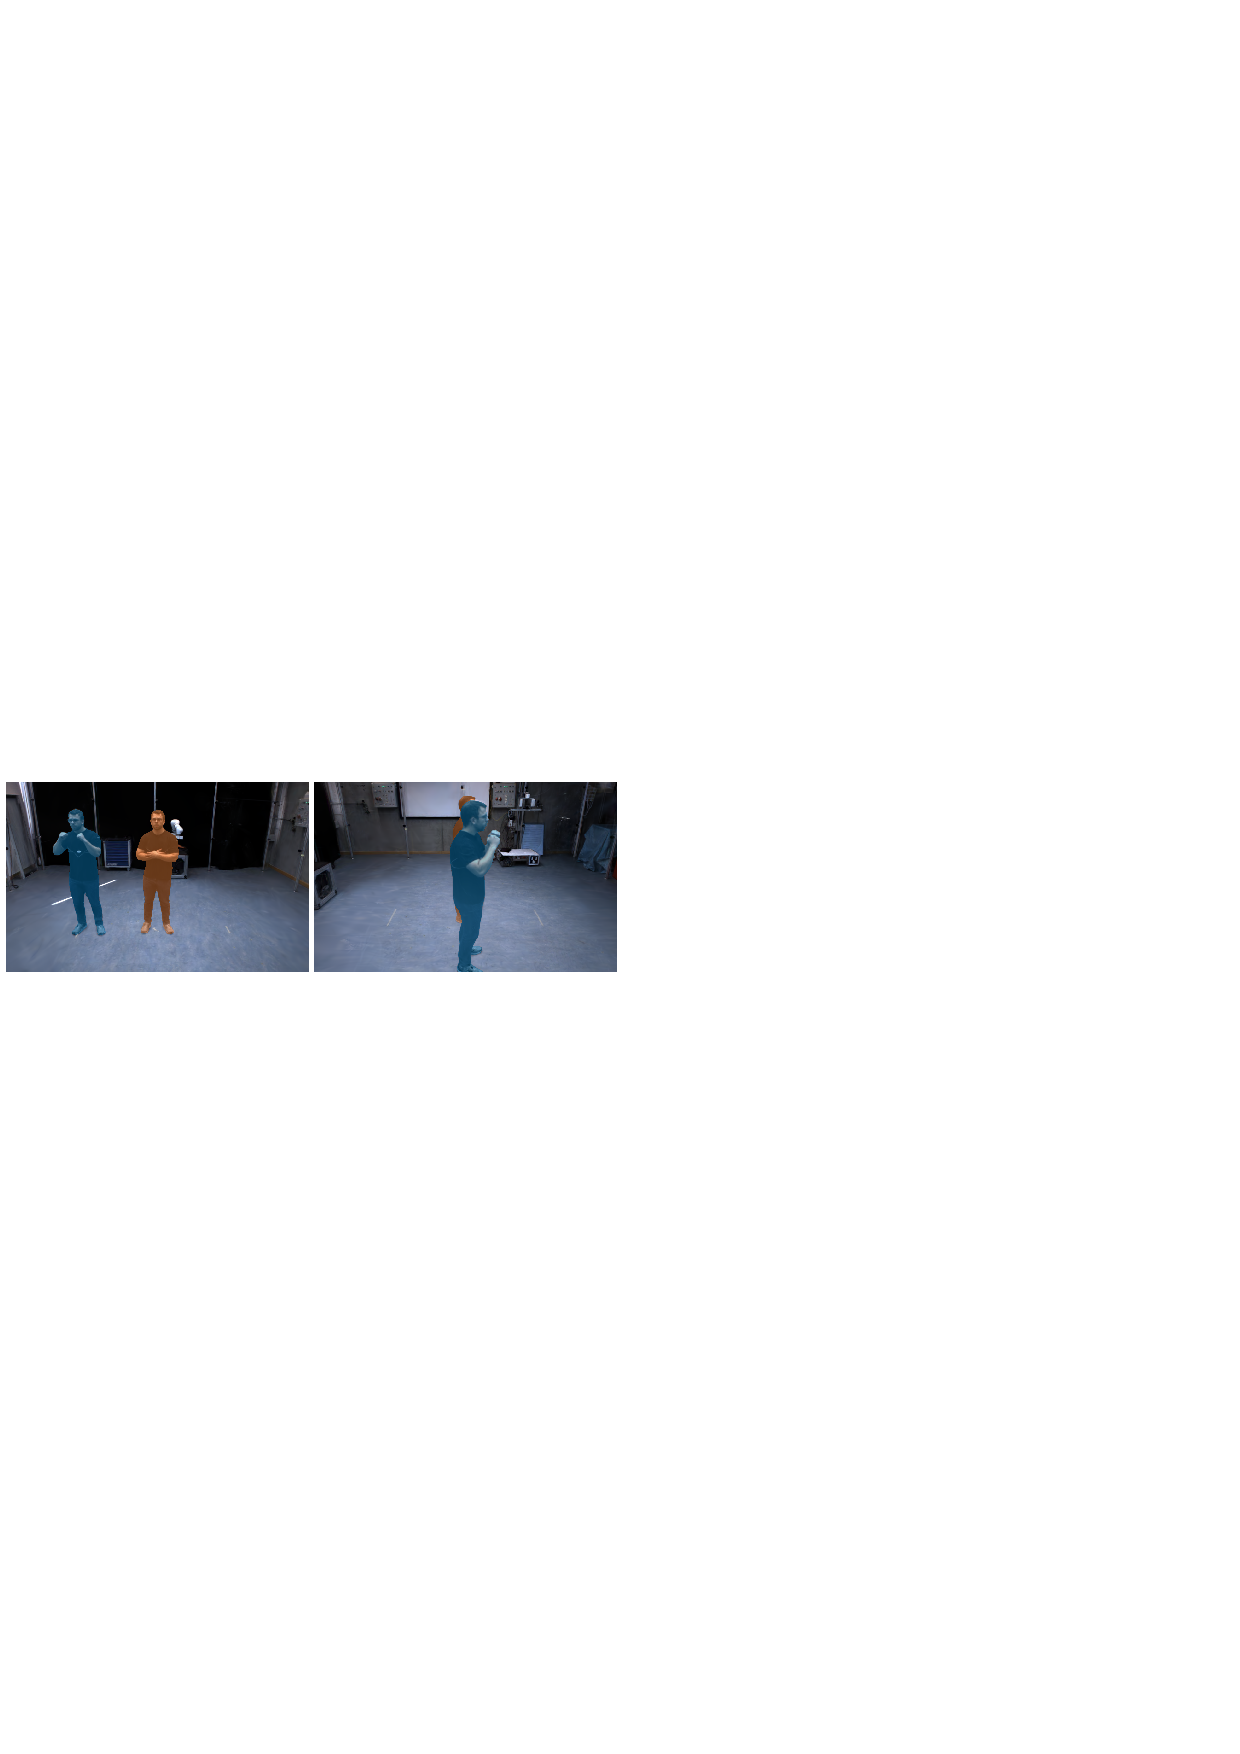
\includegraphics[width=\linewidth]{Grafiken/Oclusion.pdf}
    \caption{
        \textbf{Occlusion handling across views.}
        Segmentation overlays from front and side viewpoints of two interacting subjects.
        Even under strong mutual occlusion, instance masks remain consistent and well aligned with visible contours.
    }
    \label{fig:occlusion}
\end{figure}

\section{Scene Generalization}
Figure~\ref{fig:generalization} demonstrates the adaptability of the proposed system by recontextualizing dynamic subjects within a novel virtual environment reconstructed from real imagery using COLMAP \cite{schoenberger2016sfm}. 
The reconstructed environment provides realistic geometry and camera poses that serve as a spatial reference for compositing. 
Dynamic subjects are seamlessly integrated into the new setting, maintaining correct spatial alignment, depth consistency, and segmentation coherence. 
By decoupling object-level Gaussian models from a specific environment, the system enables arbitrary recombination of dynamic and static assets across scenes without retraining. 
This generalization capability supports large-scale variation in scene composition and facilitates applications such as domain adaptation, robustness evaluation, and synthetic-to-real transfer.

\begin{figure}[ht]
    \centering
    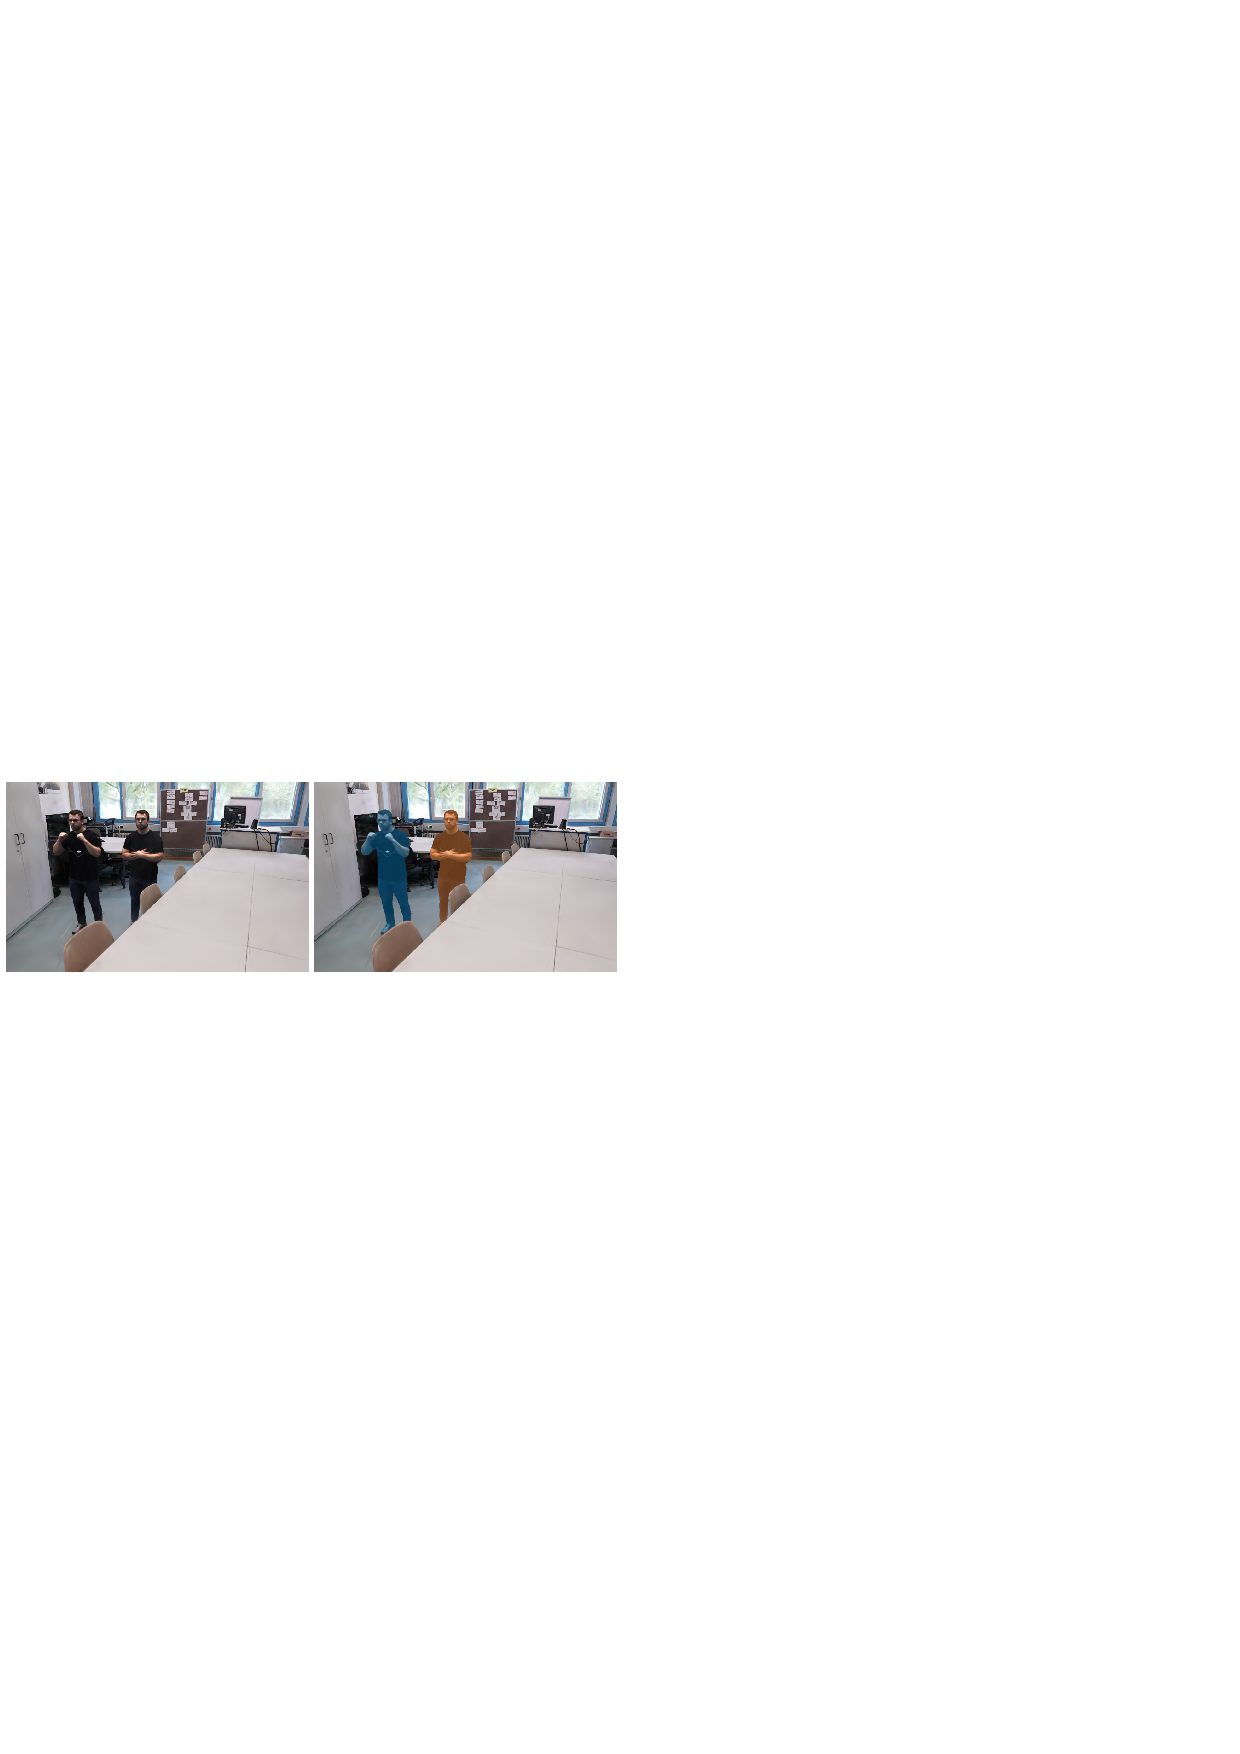
\includegraphics[width=\linewidth]{Grafiken/room_transfer.pdf}
    \caption{
        \textbf{Scene generalization and recontextualization.}
        Dynamic subjects composited into a novel virtual environment reconstructed with COLMAP.
        The system maintains consistent geometry and segmentation alignment across domains, 
        demonstrating flexible recontextualization of pre-trained Gaussian models.
    }
    \label{fig:generalization}
\end{figure}

\section{Temporal Consistency in Dynamic Scenes}
Dynamic scene rendering enables the generation of temporally coherent 4D datasets suitable for applications such as activity recognition, pose estimation, or motion segmentation. 
Figure~\ref{fig:temporal} shows representative frames from a dynamic sequence of a moving subject. 
The RGB and segmentation overlays reveal smooth and consistent motion over time, with stable geometry and accurate alignment across frames. 
Each time step preserves object structure and surface continuity, indicating that the Gaussian-based transformation updates produce interpretable and stable temporal behavior. 
This capability allows scalable synthesis of realistic dynamic sequences without requiring explicit motion capture or manual supervision.

\begin{figure*}[t]
    \centering
    \includegraphics[width=\textwidth]{Grafiken/time.pdf}
    \caption{
        \textbf{Dynamic scene generation.}
        Representative time steps of a moving subject with RGB and segmentation overlays.
        The consistent motion and geometry across frames demonstrate temporally stable 4D rendering.
    }
    \label{fig:temporal}
\end{figure*}

\section{Qualitative Pose Estimation}
Figure~\ref{fig:keypoints} (top row) shows qualitative 6D pose estimates for a dynamic human sequence across four time steps. 
Each frame visualizes the canonical object coordinate system derived from the aggregated Gaussian transformations. 
Although no ground-truth pose data are available, the estimated coordinate axes evolve consistently and reflect plausible orientation changes relative to the subject’s motion. 
This indicates that Gaussian-based transformation tracking provides a reliable approximation of object-level motion, suitable for downstream tasks such as pose refinement or motion analysis.

\section{Keypoint Propagation}
The lower row of Figure~\ref{fig:keypoints} visualizes the temporal keypoint propagation results obtained with a Detectron2-based detector \cite{Detectron22020}. 
Initial 2D keypoints are detected in a reference frame and projected into 3D by associating them with the nearest Gaussian centroids of the corresponding subject. 
As a result, keypoints are anchored on the object surface rather than the true anatomical joints, but they remain spatially coherent throughout the sequence. 
The keypoints are subsequently propagated in time according to the motion of the underlying Gaussians.

Temporal stability is observed across most body regions, particularly in the upper body where Gaussian density is high and motion is well captured. 
Minor deviations appear in areas with sparse or unstable Gaussian coverage, such as the knees or hips, leading to small temporal inconsistencies or spatial offsets. 
Despite these limitations, the propagation maintains overall semantic coherence and demonstrates that the Gaussian-based motion field can sustain meaningful correspondences over time. 
This behavior provides a promising foundation for future integration with articulated motion priors or learned joint-space constraints.

\begin{figure*}[t]
    \centering
    \includegraphics[width=\textwidth]{Grafiken/keypoints.pdf}
    \caption{
        \textbf{Qualitative analysis of pose and keypoint propagation.}
        Four frames of a dynamic subject showing estimated object poses (top) and propagated keypoints (bottom).
        The coordinate systems evolve consistently over time, while keypoint trajectories remain coherent despite local misalignments.
    }
    \label{fig:keypoints}
\end{figure*}

% \section{Summary}
% Overall, these qualitative results highlight that our framework can produce temporally stable geometric and semantic representations for dynamic scenes. 
% Although both pose and keypoint estimation currently rely on unsupervised tracking without ground-truth reference, the observed consistency across time demonstrates the potential of our 4D Gaussian representation as a foundation for future work in motion analysis, activity recognition, and articulated model learning.



 % Externe Datei einbinden
%\input{Kapitel/5_Comparison} % Externe Datei einbinden
\chapter{Summary and Outlook}

\section{Summary of Key Findings}

This work presented a modular and methodologically transparent pipeline for multi-view dataset generation based on static and dynamic 3D Gaussian Splatting representations.
Leveraging a purpose-built, hardware-synchronized multi-camera system, temporally aligned image sequences were captured from which both static (3DGS) and dynamic (D3DGS) models were reconstructed.
By integrating promptable segmentation (SAM2) and temporal mask propagation into the reconstruction workflow, all exported object models achieve geometric precision, temporal stability, and direct compatibility with downstream compositing.

A central contribution of the proposed system is the unified treatment of static and dynamic Gaussian models within a single compositional framework.
Pipeline~B enables deterministic scene assembly in calibrated camera rigs, producing spatially and temporally coherent outputs including RGB, depth, and instance-level masks.
By explicitly modeling occlusion, object placement, and temporal interpolation, the pipeline allows full control over rendered datasets while maintaining photometric and geometric realism.
This structure bridges the gap between reconstruction-focused Gaussian pipelines and practical dataset generation tools, supporting reproducible, multi-object scenes with synchronized multimodal annotations.

The framework further supports the seamless integration of externally generated 3D assets—such as those exported from \emph{Trellis}—demonstrating that pre-trained or lightweight 3D models can function as first-class entities within Gaussian-based rendering and composition.
As a result, the system generalizes across input modalities, accommodating both data-driven and generative 3D sources without modifications to the rendering logic.

\section{Limitations}

Despite its flexibility, several limitations should be acknowledged.
First, dynamic reconstructions rely on per-frame segmentation masks that, despite prompt propagation, may accumulate small temporal inconsistencies under strong occlusions or motion blur.
This can result in slight spatial drift of reconstructed Gaussians and propagated keypoints, particularly in regions with sparse Gaussian coverage such as knees or hips.

Second, although the compositional framework supports both static and dynamic elements, all rendered scenes currently assume rigid camera calibration and fixed illumination.
Consequently, phenomena such as global illumination, specular reflections, or cast shadows between independently rendered objects are not explicitly modeled, which can limit realism in certain composite configurations.

Third, pose estimation for dynamic objects is derived from Gaussian trajectories rather than explicit joint-based motion models.
While this approach ensures coherent motion propagation, it lacks semantic interpretability and may diverge from true skeletal motion.

Finally, the current implementation is optimized for controlled laboratory captures using pre-calibrated multi-camera rigs.
Generalizing to in-the-wild or handheld capture setups would require additional mechanisms to handle calibration drift, synchronization errors, and varying illumination conditions.

\section{Future Developments and Research Perspectives}

Several avenues remain open for further exploration.
A natural extension involves integrating articulated motion priors and skeleton-aware Gaussian tracking, which could improve alignment of dynamic keypoints and enable physically interpretable pose propagation.
Embedding such priors directly into the D3DGS training or composition stages may strengthen temporal coherence in regions with complex non-rigid motion, such as human limbs or deformable surfaces.

Another promising direction involves scaling the capture and synthesis process toward larger and more diverse datasets.
Automated scene composition, dynamic lighting control, and procedural environment synthesis could further enhance realism and diversity while maintaining annotation consistency.
In parallel, coupling Gaussian-based scene representations with diffusion-based appearance refinement or NeRF-style volumetric augmentation may bridge the remaining visual gap between synthetic and real-world imagery.

Finally, establishing standardized benchmarks for evaluating compositional and temporal consistency in Gaussian-rendered datasets would be highly beneficial.
Such benchmarks could promote reproducibility, enable quantitative analysis of temporal stability, and help define a common evaluation protocol for future research in Gaussian-based dataset generation.

Overall, this work demonstrates that temporally consistent Gaussian representations—when combined with geometry-aware compositing and transparent annotation pipelines—provide a practical and extensible foundation for the next generation of large-scale, multi-view training datasets. % Externe Datei einbinden
%\input{kapitel/kapitel5} % Externe Datei einbinden


\newpage

% Listen wenn überhaupt ans Ende und nicht an den Anfang.
% Meist ist das aber unnötig.
% \listoffigures % Liste der Abbildungen 
% \listoftables % Liste der Tabellen
% \newpage

\bibliographystyle{plain} % Literaturverzeichnis
% \bibliography{references}

\begin{btSect}{thesis} % mit bibtopic Quellen trennen
\addcontentsline{toc}{chapter}{Literaturverzeichnis}
\section*{Literaturverzeichnis}
\btPrintCited
\end{btSect}

% dann mit "bibtex thesis1" und "bibtex thesis2" arbeiten

\end{document}
;;; Local Variables:
;;; ispell-local-dictionary: "de_DE-neu"
;;; End:
